%%%%%%%%%%%%%%%%%%%%%%%%%%%%%%%%%%%%%%%%%%%%%%%%%%%%%%%%%%%%%%%%%%%%%%%%%%%%%%%%
\documentclass[twocolumn]{revtex4}

%%%%%%%%%%%%%%%%%%%%%%%%%%%%%%%%%%%%%%%%%%%%%%%%%%%%%%%%%%%%%%%%%%%%%%%%%%%%%%%%
% Note that comments begin with a "%" and are not turned into text in the .pdf
% document.
%%%%%%%%%%%%%%%%%%%%%%%%%%%%%%%%%%%%%%%%%%%%%%%%%%%%%%%%%%%%%%%%%%%%%%%%%%%%%%%%

%%%%%%%%%%%%%%%%%%%%%%%%%%%%%%%%%%%%%%%%%%%%%%%%%%%%%%%%%%%%%%%%%%%%%%%%%%%%%%%%
% Include some extra packages.
%%%%%%%%%%%%%%%%%%%%%%%%%%%%%%%%%%%%%%%%%%%%%%%%%%%%%%%%%%%%%%%%%%%%%%%%%%%%%%%%
\usepackage[]{graphicx}
%%%%%%%%%%%%%%%%%%%%%%%%%%%%%%%%%%%%%%%%%%%%%%%%%%%%%%%%%%%%%%%%%%%%%%%%%%%%%%%%

%%%%%%%%%%%%%%%%%%%%%%%%%%%%%%%%%%%%%%%%%%%%%%%%%%%%%%%%%%%%%%%%%%%%%%%%%%%%%%%%
\begin{document}

%%%%%%%%%%%%%%%%%%%%%%%%%%%%%%%%%%%%%%%%%%%%%%%%%%%%%%%%%%%%%%%%%%%%%%%%%%%%%%%%
\title{ Will You Be Eaten By a 'Raptor?
}

\author{S.~Mainella}
\author{M.~Bellis}
\affiliation{Siena College, Loudonville, NY}

\date{\today}

\begin{abstract}
   This final project was a build-off of the midterm project and continues the battle between you and the velociraptor. The main goals were to plot a graph of the speeds of a velociraptor and you, determine how far and how much time has passed when the velociraptor catches up to you, plot how close enough the velociraptor is to attack, and what the probability is of you surviving. It took the velociraptor 2 seconds to catch up to the person running 6 meters and had a 30 meter start. It took the velociraptor 1.93 seconds to reach striking distance to the person running 5.8 meters and had a 30 meter start. You have a 62\% of surviving from three attack attempts of the velociraptor.
\end{abstract}

\maketitle
%%%%%%%%%%%%%%%%%%%%%%%%%%%%%%%%%%%%%%%%%%%%%%%%%%%%%%%%%%%%%%%%%%%%%%%%%%%%%%%%

%%%%%%%%%%%%%%%%%%%%%%%%%%%%%%%%%%%%%%%%%%%%%%%%%%%%%%%%%%%%%%%%%%%%%%%%%%%%%%%%
\section{Question 1}
\centering
    Question 1 asks to plot a position versus time graph of you and the velociraptor. I have constructed a graph using two equations. This equation represents the speed of a velociraptor:
     $$y_0=18x$$
     This equation represents your speed and 30 meter head start:
     $$y_1=3x+30$$
     In order to construct this graph, I had to import matplotlib.pylab, numpy, and matplotlib.incline. To create my lines, I used 'linspace' for x to generate the amount of evenly spaced points for the equation. I edited the axes to make the intersection more visible.

\begin{figure}[h!]
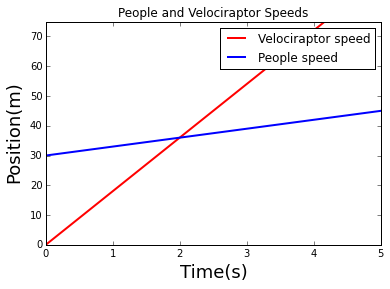
\includegraphics[width=0.5\textwidth]{v1.png}



\end{figure}
\pagebreak
%%%%%%%%%%%%%%%%%%%%%%%%%%%%%%%%%%%%%%%%%%%%%%%%%%%%%%%%%%%%%%%%%%%%%%%%%%%%%%%%

\section{Question 2}
\centering
Question 2 asks, "When does the 'raptor catch up to you.?" I made a function and called it 'intersection.' Intersection brings in the two lines and 'x'. In the function theres a for loop that consists of all the points linspace created off of the two equations. I used an if statement saying if the point of each line is equal to each other, return that coordinate. The 'x' value returns the time the 'raptor caught up to you, and the 'y' value returns how many meters you've ran. 30 must be subtracted by the 'y' coordinate because that is the value of your origin. Here is an algebraic approach to find the intersection:
$$y_0=18x \quad   y_1=3x+30$$
$$  18x=3x+30$$
$$ 15x=30$$
$$x=2$$
$$18(2)=3(2)+30$$
$$y=36 \quad 36- 30$$
$$y=6$$



\pagebreak
%%%%%%%%%%%%%%%%%%%%%%%%%%%%%%%%%%%%%%%%%%%%%%%%%%%%%%%%%%%%%%%%%%%%%%%%%%%%%%%%
\section{Question 3}

A 'raptor will start trying to attack you when it is 1 meter away. Question 3 asks, "When is it close enough to strike?" I used a procedure similar to the one in Question 2. The function, strikeintersection, takes in the 2 lines and 'x,' again. Rather than having an if statement that sets the two points of the lines equal to each other, I set the difference of the two lines to be less than 1. 1 represents the meter away the 'raptor is to you. The function returns the coordinates of when the 'raptor is in striking distance. Again, 30 must be subtracted by the 'y' coordinate because that is the value of your origin.  

\begin{figure}[h!]
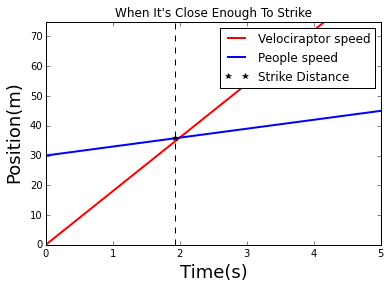
\includegraphics[width=0.5\textwidth]{strike.png}
\end{figure}
To solve this problem algebraically, I found the intersection between the two equations by adding 1 to the velociraptor speed equation like so:

$$y_0=18x+1 \quad y_1=3x+30$$
$$18x+1=3x+30$$
$$15x=29$$ 
$$x=1.93$$
$$18(1.93)+1=3(1.93) +30$$
$$y=35.8 \quad 35.8 - 30$$
$$y=5.8$$

\pagebreak






%%%%%%%%%%%%%%%%%%%%%%%%%%%%%%%%%%%%%%%%%%%%%%%%%%%%%%%%%%%%%%%%%%%%%%%%%%%%%%%%
\section{Question 4}
Question 4 asks what is the probability you survive after three velociraptor attack attempts. There is a 20 \% chance it will eat you on its first try. If the 'raptor misses its first attempt, there is a 15 \% chance it will eat you on its second try. If the 'raptor misses the second attempt, there is a 7 \% chance it will eat you on its third try. In order to solve this probability equation, I used a nested conditional and a Monte Carlo calculation. 'npts' represents the amount of points I used for the conditional. The more points used makes the calculation more accurate. I set 'x' to a random number generator. Then, I made a for loop that ranges from 0 to my 'npts.' First try is all of the random numbers generated from 0-1. I made an if statement that will take out all of those numbers of which are greater than .2. I called these numbers 'second.' Of the random numbers that are greater than .2, I made another if statement taking out all of those numbers of which are greater than .15. I called these numbers 'third.' The last if statement takes out all of the numbers of which are greater than .7. 'p' is the number of successful times of you surviving. It must be set to zero before the nested conditional because neither you nor the 'raptor has run yet. After the loop and conditional have run, the equation, p = p + 1 records how many times you have survived out of 'npts' times. When this is recorded, I wrote a simple part/whole equation to get the fraction. I multiplied the fraction by 100 and got the percent answer.
%%%%%%%%%%%%%%%%%%%%%%%%%%%%%%%%%%%%%%%%%%%%%%%%%%%%%%%%%%%%%%%%%%%%%%%%%%%%%%%%
\end{document}
%%%%%%%%%%%%%%%%%%%%%%%%%%%%%%%%%%%%%%%%%%%%%%%%%%%%%%%%%%%%%%%%%%%%%%%%%%%%%%%%
